\documentclass[printmode, eng, openany]{mgr}
\usepackage{polski}
\usepackage[utf8]{inputenc}
\usepackage[T1]{fontenc}

\usepackage{graphicx}
\usepackage{subfigure}
\usepackage{psfrag}
\usepackage{float}

\usepackage{amsmath}
\usepackage{amsfonts}


\usepackage{supertabular}
\usepackage{array}
\usepackage{tabularx}
\usepackage{hhline}

\usepackage{hyperref}
\usepackage{listings}
\hypersetup{
    colorlinks=true,
    linkcolor=black,
    filecolor=black,      
    urlcolor=black,
}
\newtheorem{theorem}{Twierdzenie}[section]

\title{Projekt i implementacja aplikacji automatycznej klasyfikacji utworów muzycznych z różnych epok}
\engtitle{Design and implementation of the application for process of automatic classification of classical music from different eras}
\author{Patryk Grzybała}
\supervisor{dr inż. Maciej Walczyński, PWr}
\field{Elektronika (EKA)}
\specialisation{Inżynieria akustyczna (EIA)}

\newcommand\tab[1][1cm]{\hspace*{#1}}
\newcommand*\rfrac[2]{{}^{#1}\!/_{#2}}

\linespread{1.3}
\begin{document}
\maketitle

\tableofcontents

\chapter{Wstęp}
\tab Celem pracy było stworzenie aplikacji pozwalającej na klasyfikację klasycznych utworów muzycznych z wykorzystaniem algorytmów uczenia maszynowego oraz formatu\linebreak MusicXML.\\
\tab W niniejszej pracy inżynierskiej omawiany jest temat automatycznego rozpoznawania utworów muzyki klasycznej z różnych epok wykorzystując do tego algorytmy uczenia maszynowego. Praca omawia wyniki uzyskane podczas tworzenia aplikacji oraz omawia napotkane problemy podczas jej tworzenia. \\

\tab Uczenie maszynowe zyskuje na coraz większej popularności. Uczenia maszynowe jako dziedzina nauk o sztucznej inteligencji pojawiła się już w latach pięćdziesiątych ubiegłego wieku kiedy Arthur Lee Samuel po raz pierwszy, w roku 1959, użył terminu "uczenie maszynowe". Program Arthura uczył się grać w prostą grę planszową - warcaby. W kolejnych latach dzięki uczeniu maszynowemu odkryto nieznane molekuły związków organicznych, a wyniki tychże badań ukazały się w prasie naukowej i po raz pierwszy nie były to badania wykonane przez człowieka. Obecnie uczenie maszynowe jest wykorzystywane w wielu dziedzinach z ogromnymi sukcesami.
\section{Zakres pracy}
\tab W zakres pracy wchodzą:
\begin{itemize}
\item pozyskanie parametrów opisujących utwór muzyczny z plików MusicXML pozwalających na reprezentowanie zachodniej notacji muzycznej,
\item stworzenie bazy danych plików muzycznych z podziałem na różne epoki,
\item wykorzystanie istniejących algorytmów uczenia maszynowego do jak najlepszej klasyfikacji utworów muzycznych,
\item stworzenie interfejsu wiersza poleceń pozwalającego na sklasyfikowanie utworu.
\end{itemize}
\section{Zawartość pracy}
\tab Rozdział 2 ("Muzyka klasyczna") opisuje pokrótce epoki w muzyce oraz skupia się na zapisie nutowym.\\
\tab Rozdział 3 ("Baza plików muzycznych MusicXML") mówi o tworzeniu bazy plików muzycznych wykorzystywanych do późniejszej nauki klasyfikatorów uczenia maszynowego oraz o formacie MusicXML.\\ 
\tab Rozdział 4 ("Uczenie maszynowe") zawiera podstawowe informacje o uczeniu maszynowym, jego rodzajach, niektórych algorytmu klasyfikujących oraz wstępnym przetwarzaniu danych.\\ 
\tab Rozdział 5 ("Implementacja aplikacji") przedstawia środowisko w jakim została napisana aplikacja, omawia w skrócie bibliotekę \textit{music21} oraz opisuje jak została stworzona aplikacja.\\ 
\tab Rodział 6 ("Podsumowanie") omawia uzyskane wyniki klasyfikacji, wnioski, które nasunęły się podczas pisania pracy oraz możliwości rozwoju czy usprawnienia aplikacji. \\ 
\chapter{Muzyka klasyczna}
\tab Muzyka towarzyszyła nam od czasów prehistorycznych, grano podczas ceremonii religijnych oraz do zabawy. Najstarszy wiernie odtworzony utwór muzyczny pochodzi\linebreak z państwa Hurytów, jest to "Hymn do Nikkal" i datowany jest na rok 1400 p.n.e., natomiast najstarszy kompletny utwór muzyczny, który zachował się do czasów współczesnych datowany jest na XI wiek.
\section{Epoki w muzyce klasycznej}
\subsection{Średniowiecze}
\tab Muzyka w średniowiecznej Europie nie była czymś pospolitym. Muzykę uważano za naukę, a także większość autorów nie podpisywała się pod swoimi dziełami, miała na to wpływ filozofia małości człowieka wobec Boga. W hierarchii społecznej teoretycy muzyczni zajmowali znacznie większą pozycję niż kompozytorzy, ci ostatni byli tylko rzemieślnikami. \\
\tab W końcówce IX wieku zaczęła pojawiać się notacja muzyczna służąca do zapisu chorału gregoriańskiego zwana notacją neumatyczną. Znaki w tej notacji odpowiadały pojedynczym dźwiękom albo ich grupom. Umieszczano je nad tekstem śpiewanym. Miało to określić przybliżony kształt melodii. \\
\tab Guido z Arezzo wprowadził do tej notacji dwie równoległe linie i dwie litery C - przy wyższej linii oraz F przy niższej linii. Litery te oznaczały wysokość dźwięku zapisanych na danych liniach. W późniejszych latach, pod koniec XI wieku, dodano dwie, a następnie jeszcze jedną linię. Tak narodziła się znana nam ówcześnie pięciolinia.
\subsection{Renesans}
\tab Za początek renesansu w muzyce uznaje się rok 1400, kiedy zaczęto wykorzystywać nieznane w średniowieczu techniki kompozytorskie. Muzyka tego okresu była przeznaczona głównie dla bogatego mieszczaństwa oraz na dwory władców. Zaczynają się pojawiać utwory świeckie: pieśni miłosne, madrygały i utwory okolicznościowe. Muzyka zmieniła swój status z nauki na sztukę. \\
\tab Wśród muzyki sakralnej dominowały msze i motety, natomiast w muzyce świeckiej dominował chanson oraz madrygał. Główne instrumenty utożsamiane z renesansem to puzon, lutnia, viola da gamba oraz organy. \\
\tab Dodatkowym czynnikiem rozwijającym muzykę renesansową było wynalezienie maszyny drukarskiej co pozwoliło na proste kopiowanie nut i rozpowszechnienie muzyki na większą skalę.
\subsection{Barok}
\tab W roku 1600 nastąpił przełom w muzyce, gdy we Florencji wystawiono pierwsze zachowane dzieło operowe "Dramma per musica" Jacopo Periego. Przyczyniło się to do powstania nowego gatunku - opery. Nowa epoka w muzyce miała odróżniać się od  poprzedniej przede wszystkim jej ekspresywnością i indywidualnym charakterem. Muzyka baroku miała za zadanie wyrażanie emocji, a także pobudzanie w słuchaczu uczuć zwanych afektami.\\
\tab Na przełomie XVII i XVIII wieku muzyka stawała się bardziej monumentalna. Utwory były coraz dłuższe, wieloczęściowe, były wykonywane przez większą ilość muzyków. Muzyka instrumentalna bardzo się rozwijała, w tym okresie powstały między innymi sonaty oraz koncerty solowe jako gatunki. Warto również wymienić tu nazwiska takich twórców jak Antonio Vivaldi, Jerzy Fryderyk Händel oraz Jan Sebastian Bach, którzy są ikonami muzyki z tamtego okresu.\\
\subsection{Klasycyzm}
\tab Za początek klasycyzmu uznaje się śmierć Jana Sebastiana Bacha w roku 1750. Do najbardziej znanych kompozytorów z tego okresu należeli Józef Haydn, Wolfgang Amadeusz Mozart, a także Ludwig van Beethoven oraz Franz Schubert, których twórczość ciężko jednak przypisać jednoznacznie do okresu klasycyzmu, gdyż są pionierami również epoki romantycznej.\\
\tab W epoce klasycyzmu udoskonalano gatunki i formy, takie jak sonaty, symfonie, koncerty czy kwartety. Jest to epoka bardzo różnorodna posiadająca wiele szkół i stylów. Początek tej epoki to przede wszystkim styl \textit{galant}, muzyka w tym stylu miała być przyjemna, prosta ale też elegancka, a jej głównym zadaniem było wprowadzenie słuchacza\linebreak w dobry nastrój. Kompozytorzy rezygnowali z polifonii, która była wszechobecna w stylu barokowym. 
\subsection{Romantyzm}
\tab XIX wiek był rozkwitem nurtu romantycznego w Europie, rozpoczynając od nazwiska Ludwiga van Beethovena, w którego muzyka ukształtowała późniejszych twórców romantycznych. XIX był też początkiem twórczości wirtuozowskiej - \textit{brillant}. Głównymi inspiracjami muzyki tego okresu był folklor, egzotyka, natura, filozofia, literatura oraz inne sztuki. Odmienił się status społeczny kompozytora i wykonawcy, a także muzyki\linebreak w pojmowaniu społeczeństwa. Publiczne koncerty stawały się coraz bardziej popularne.\\
\tab Romantyczni twórcy starali się tworzyć swoje unikatowe style, odchodzono od szeroko przyjętych schematów form muzycznych i zasad porządkujących przebieg dzieła muzycznego. Gatunki muzyczne nie były tak dystynktywne. Teksty utworów romantycznych często były poświęcone tematom miłości oraz samotności, a inspiracją do nich była twórczość ówczesnych poetów.
\subsection{XX wiek}
\tab Muzyka XX wieku stanowi bunt wobec muzyki z wcześniejszych okresów. Charakteryzuje się poszukiwaniem nowości, inności oraz łamaniem zasad. Poprzednie epoki odznaczały się tzw. \textit{tonalnością funkcyjną} co oznacza, że panowała w nich swego rodzaju hierarchia, zdarzenia muzyczne były skorelowane z tym co działo się wcześniej, a także pozwalały przewidywać co stanie się później. Uznano jednak, należy szukać nowych zasad. Jednak cechą, która łączy muzykę wieku XX z muzyką lat poprzednich były uprawiane formy i gatunki muzyczne takie jak symfonie czy opery. Muzyka tego okresu jest bardzo zróżnicowana.
\section{Zapis nutowy}
\tab W tej pracy pliki wykorzystane do klasyfikacji zawierają między innymi informacje o wysokości dźwięku i wartości rytmiczne nut, są to dwie główne informacje wykorzystane do parametryzacji utworów muzycznych.
\subsection{Wysokość dźwięku}
\tab Wysokość dźwięku danej nuty określa jej częstotliwość tonu podstawowego. Na partyturze wysokość dźwięku danej nuty określa jej położenie na pięciolinii, klucz oraz znaki chromatyczne, czyli krzyżyki, bemole i kasowniki.\\ W tabeli 2.1 przedstawiono ilość drgań dla dźwięków w oktawie razkreślnej.

\begin{table}[!htb]
\centering
\caption{Dzwięki i ich częstotliwości w oktawie razkreślnej}
\begin{tabular}{|l|c|c|c|c|c|c|c|c|}
\hline
Dźwięk & $c^{1}$ & $d^{1}$ & $e^{1}$ & $f^{1}$ & $g^{1}$ & $a^{1}$ & $h^{1}$ & $c^{2}$  \\
\hline
Częstotliwość [Hz] & 261,6 & 293,7 & 329,6 & 349,2 & 391,9 & 440,0 & 493,9 & 523,2 \\
\hline
\end{tabular}
\end{table}
\subsubsection{Klucz}
\tab Klucz, umieszczany na początku pięciolinii, przyporządkowuje liniom odpowiednie wysokości dźwięków. Istnieją trzy rodzaje kluczy G, F oraz C, które zostały zaprezentowane odpowiednio na rysunkach 2.1, 2.2 oraz 2.3.

\begin{figure}[!htb]
\begin{minipage}{0.31\textwidth}
\centering
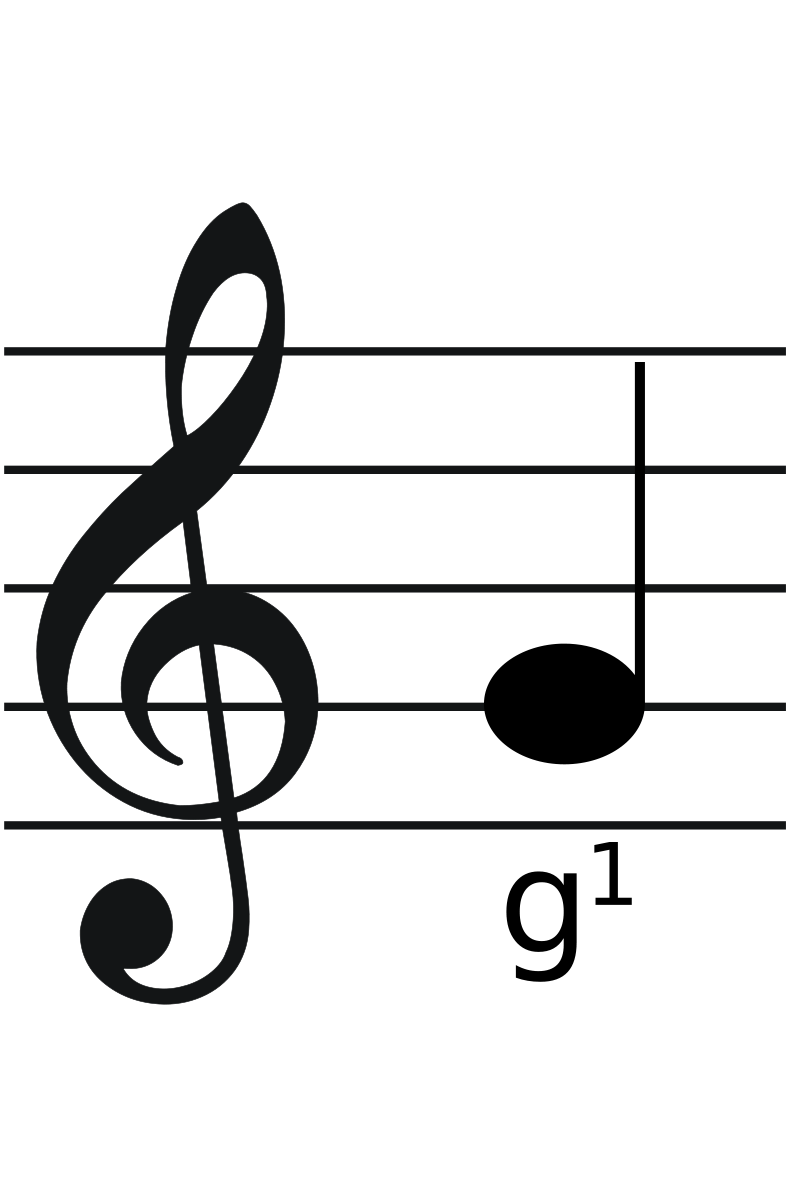
\includegraphics[width=3cm]{G}
\caption{Klucz G.}
\end{minipage}
\begin{minipage}{0.31\textwidth}
\centering
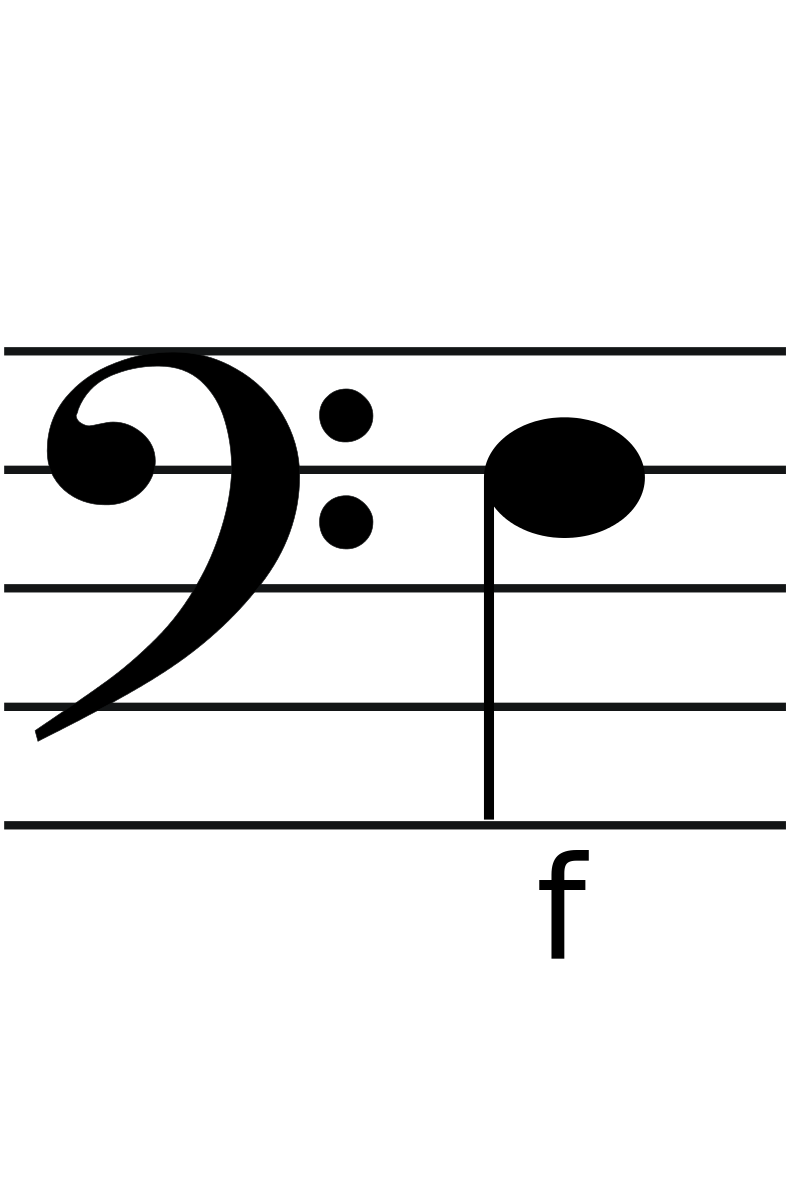
\includegraphics[width=3cm]{F}
\caption{Klucz F.}
\end{minipage}
\begin{minipage}{0.31\textwidth}
\centering
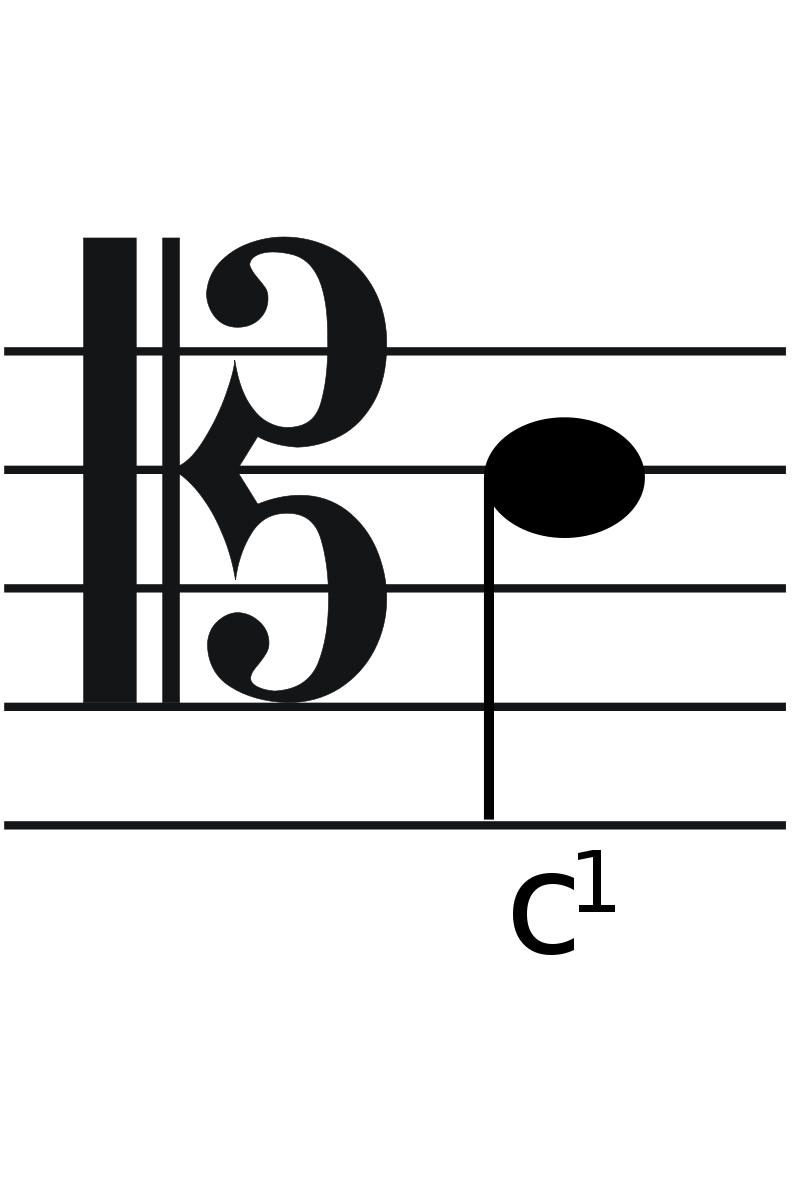
\includegraphics[width=3cm]{C}
\caption{Klucz C.}
\end{minipage}
\end{figure}

\tab Klucz G wskazuje położenie dźwięku $g^{1}$, klucz F wskazuje położenie dźwięku\linebreak$f$, a klucz C położenie dźwięku $c^{1}$ na pięciolinii. Klucze ułatwiają zapis dźwięków na odpowiednie partie, na przykład nuty dla instrumentów nisko brzmiących takich jak kontrabas zapisuje się z użyciem klucza basowego, a klucza wiolinowego używa się do zapisu nut dla wysoko brzmiących skrzypiec. Inaczej pięciolinia nie wystarczyłaby do zapisu wszystkich dźwięków, nawet z liniami dodatkowymi.

\subsubsection{Krzyżyk}
\tab Krzyżyk podnosi dźwięk o pół tonu, czyli sprawia, że dźwięk jest podniesiony\\o $\sqrt[12]{2}$ raza.
\begin{figure}[!htb]
\centering
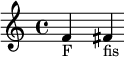
\includegraphics[width=3.6cm]{krzyzyk.png}
\caption{Symbol krzyżyka przy nucie.}
\end{figure}

\subsubsection{Bemol}
\tab Bemol jest przeciwieństwem krzyżyka i obniża dźwięk o pół tonu.
\begin{figure}[!htb]
\centering
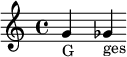
\includegraphics[width=3.6cm]{bemol.png}
\caption{Symbol bemolu przy nucie.}
\end{figure}

\subsubsection{Kasownik}
\tab Kasownik, jak sama nazwa wskazuje, kasuje znaczenie wyżej wymienionych znaków chromatycznych. Postawienie np. bemolu przed nutą G oznacza, że wszystkie nuty\linebreak G w danym takcie będą obniżone o pół tonu staną się nutami ges, z kolei postawienie kasownika przed nutą ges kasuje znaczenie bemolu i dźwięk zostaje podniesiony o pół tonu w górę. Ilustruje to rysunek 2.6.

\begin{figure}[!htb]
\centering
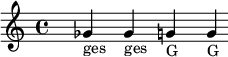
\includegraphics[width=6cm]{kasownik_poj}
\caption{Zmiana tonu dzwięku ges przez kasownik.}
\end{figure}

\tab Znaki chromatyczne można jednak stawiać także za kluczem, obowiązują wtedy w całym utworze lub są tymczasowo usuwane przez kasownik.

\subsection{Wartości nut}
\tab Wartości rytmiczne nut określają długość ich trwania. Podstawową jednostką jest \textit{cała nuta}, według której określone są pozostałe nuty. Cała nuta nie ma absolutnie zdefiniowanego czasu trwania, jest on definiowany przez \textit{tempo} utworu. Cała nuta trwa pełny takt w metrum $\rfrac{2}{2}$ czy $\rfrac{4}{4}$. Cała nuta zawiera dwie półnuty, cztery ćwierćnuty, osiem ósemek itd.

\begin{figure}[H]
\centering
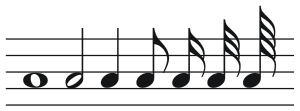
\includegraphics[width=6cm]{wartosci_nut}
\caption{Symbole nut przedstawiające różne wartości nut, kolejno od lewej: cała nuta, półnuta, ćwierćnuta, ósemka, szesnastka, trzydziestodwójka, sześćdziesięcioczwórka.}
\end{figure}
\tab Wartości rytmiczne nut mogą być zmieniane. Podobnie jak zwiększana jest wysokość dźwięku przez krzyżyki tak długość nuty może być wydłużona przez łuk lub kropkę. 
\subsubsection{Łuk}
\tab Łuk łączy dwie nuty tylko i wyłącznie o tej samej wysokości, ich wartości się sumują. Łuki łączące nuty o różnych wysokościach mają inne znaczenie. Na rysunku 2.9 zaprezentowano połączenie dwóch półnut w jedną całą nutę. Dźwięki w obu taktach brzmią tak samo.

\begin{figure}[!htb]
\centering
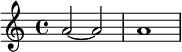
\includegraphics[width=5.4cm]{luk}
\caption{Łączenie dwóch półnut do całej nuty przez łuk.}
\end{figure}

\subsubsection{Kropka}
\tab Kropka po prawej stronie nuty wydłuża jej wartość o połowę wartości nuty przy której została napisana, to znaczy, że cała nuta z kropką trwa tyle co cała nuta i półnuta, półnuta z kropką trwa tyle co półnuta i ćwierćnuta itd. Zależność ta została zaprezentowana na rysunku 2.10. Kropka pisana nad nutą ma inne znaczenie.

\begin{figure}[!htb]
\centering
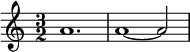
\includegraphics[width=5.4cm]{kropka}
\caption{Wydłużenie wartości całej nuty przez kropkę.}
\end{figure}

\chapter{Baza plików muzycznych MusicXML}
\tab W ramach niniejszej pracy musiała zostać stworzona baza plików muzycznych utworów z różnych epok. Pliki muzyczne zgodnie z założeniami były w formacie MusicXML\linebreak i zostały pobrane ze stron:
\begin{itemize}
\item \url{https://www.cpdl.org/wiki/}
\item \url{https://musescore.com/sheetmusic}
\end{itemize}
\section{Format MusicXML}
\tab Format MusicXML to cyfrowy format do zapisu notacji nutowej i łatwego udostępniania zachodnich utworów muzycznych. Celem tego formatu jest stworzenie uniwersalnego nośnika do udostępniania nut. Obecnie wiele programów komputerowych wspiera otwieranie plików MusicXML. Przed MusicXML jedynym powszechnie stosowanym formatem do zapisywania notacji było MIDI, jednak ten format nie wspiera wielu cech notacji nutowej. MusicXML używa języka znaczników XML do zapisu informacji, który został wybrany ze względu na niezależność od platformy i jest świetny do reprezentowania dużej ilości strukturalnych danych co wpasowuje go idealnie do reprezentacji partytury. Dodatkowym atutem tego formatu jest fakt, że nie ma potrzeby tworzenia nowych parserów tego języka, gdyż istnieją one już od dłuższego czasu.\\
\tab Pliki MucsicXML użyte podczas tworzenia bazy muzyki używają skompresowanego formatu .mxl, który pozwala zaoszczędzić około 20 razy więcej miejsca, przykładowo cztery strony nut w nieskompresowanym formacie .musicxml zajmują nawet 518kB pamięci, a przy użyciu skompresowanego formatu .mxl tylko 19kB co jest nawet mniejszą ilością w porównaniu do reprezentacji MIDI, która wynosi 21kB, a jednocześnie zawiera mniej informacji.
\subsection{Przykład pliku MusicXML}
\begin{figure}[!htb]
\centering
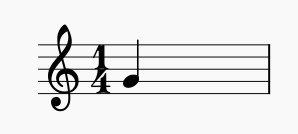
\includegraphics[width=5.4cm]{xml_example}
\caption{Przykład formatu .mxl odtworzonego za pomocą programu MuseScore 3.}
\end{figure}
\begin{lstlisting}
<?xml version="1.0" encoding="UTF-8"?>
<!DOCTYPE score-partwise PUBLIC
    "-//Recordare//DTD MusicXML 3.1 Partwise//EN"
    "http://www.musicxml.org/dtds/partwise.dtd">
<score-partwise version="3.1">
  <part-list>
    <score-part id="P1">
      <part-name>Music</part-name>
    </score-part>
  </part-list>
  <part id="P1">
    <measure number="1">
      <attributes>
        <divisions>1</divisions>
        <key>
          <fifths>0</fifths>
        </key>
        <time>
          <beats>1</beats>
          <beat-type>4</beat-type>
        </time>
        <clef>
          <sign>G</sign>
          <line>2</line>
        </clef>
      </attributes>
      <note>
        <pitch>
          <step>G</step>
          <octave>4</octave>
        </pitch>
        <duration>1</duration>
        <type>quarter</type>
      </note>
    </measure>
  </part>
</score-partwise>
\end{lstlisting}

\tab Na rysunku 3.1 przedstawiono graficzną reprezentacje powyższego kodu. Przeanalizujmy wszystkie części tego kodu.
 
\begin{lstlisting}
<?xml version="1.0" encoding="UTF-8"?>
\end{lstlisting}
Wymagana deklaracja dokumentu wszystkich plików XML, z ustalonym kodowaniem znaków na UTF-8 posiadającym zbiór znaków ASCII.

\begin{lstlisting}
<!DOCTYPE score-partwise PUBLIC
    "-//Recordare//DTD MusicXML 3.1 Partwise//EN"
    "http://www.musicxml.org/dtds/partwise.dtd">
\end{lstlisting}
Te linijki mówią o tym, że używamy MusicXML, jednocześnie specyfikujemy lokalizację DTD(ang. Document Type Definition), czyli dokumentu definiującego strukturę plików XML. Pozwala to na rozpoznanie plików MusicXML przez aplikacje.

\begin{lstlisting}
<score-partwise version="3.1">
\end{lstlisting}
To jest główny \textit{korzeń} (ang. \textit{root}) dokumentu, element <score-partwise> składa się\linebreak z części, a każda z części składa się z taktów. Atrybut elementu \textit{version} definiuje, którą wersję MusicXML używamy.

\begin{lstlisting}
<part-list>
  <score-part id="P1">
     part-name>Music</part-name>
  </score-part>
</part-list>
\end{lstlisting}
Powyższy znacznik \textit{<part-list>} jest nagłówkiem zawierającym liczbę części w partyturze, w powyższym przykładzie zawiera on tylko jeden element, który jako wymagany atrybut zawiera ID części oraz również wymagany element \textit{<part-name>} zawierający nazwę części.


\begin{lstlisting}
<part id="P1">
\end{lstlisting}
Tu zaczyna się pierwsza i jedyna część w utworze, wymagany atrybut \textit{<id>} musi odnosić się do ID zdefiniowanym w elemencie nagłówkowym \textit{<part-list>}.

\begin{lstlisting}
<measure number="1">
\end{lstlisting}
Rozpoczynamy takt numer 1.

\begin{lstlisting}
<attributes>
\end{lstlisting}
Element \textit{<attributes>} zawiera informacje potrzebne do interpretacji wartości muzycznych nut.


\begin{lstlisting}
<divisions>1</divisions>
\end{lstlisting}
Każda nuta w MusicXML zawiera swój element określający jej czas trwania. Element \textit{<divisions>} dostarcza jednostkę pomiaru długości elementu  ze względu na podział na ćwierć nuty. W tym przykładzie mamy tylko jedną ćwierćnutę o elemencie \textit{<duration>} równym 1. Element \textit{<divisions>} powinien być równy długości ćwierćnuty.

\begin{lstlisting}
<key>
   <fifths>0</fifths>
</key>
\end{lstlisting}
Element \textit{<key>} reprezentuje znaki przykluczowe, wartość 0 oznacza tonacje C-dur. Wartości pozytywne dodają krzyżyki, wartości negatywne dodają bemole. 

\begin{lstlisting}
<time>
  <beats>1</beats>
  <beat-type>4</beat-type>
</time>
\end{lstlisting}
Powyższy element oznacza metrum. Górny element \textit{<beats>} oznacza liczbę jednostek metrycznych, dolny element \textit{<beat-type>} oznacza podstawową jednostkę metryczną utworu, w tym przykładzie w takcie mamy takty o długości jednej ćwierćnuty.

\begin{lstlisting}
<clef>
  <sign>G</sign>
  <line>2</line>
</clef>
\end{lstlisting}
\textit{<clef>} definiuje klucz, MusicXML pozwala na użycie kluczy, które już nie są dziś\linebreak w użyciu. W powyższym kodzie element \textit{<sign>} oznacza typ klucza, a \textit{<line>} linijkę na której się znajduje. G2 to klucz wiolinowy.

\begin{lstlisting}
</attributes>
<note>
\end{lstlisting}
Koniec definicji atrybutów, czas na zapis nut w takcie.

\begin{lstlisting}
<pitch>
  <step>C</step>
  <octave>4</octave>
</pitch>
\end{lstlisting}
Element \textit{<pitch>} oznacza wysokość dźwięku nuty. Posiada dwa wymagane elementy \textit{<step>} i \textit{<octave>} oraz jeden opcjonalny \textit{<alter>}. Step oznacza nazwę dźwięku, a octave oktawę. Element alter reprezentuje krzyżyk lub bemol, musi zostać użyty nawet, gdy  tonacja została określona w elemencie \textit{<fifths>}.

\begin{lstlisting}
<duration>1</duration>
\end{lstlisting}
Nuta użyta w przykładzie to ćwierćnuta, a nasz element \textit{<divisions>} ma wartość 1. Co oznacza, że \textit{<duration>1</duration>} oznacza, że 1 to długość jednej ćwierćnuty. Gdyby w przykładzie użyto półnuty, element \textit{<duration>} musiałby mieć wartość 2.

\begin{lstlisting}
<type>quarter</type>
\end{lstlisting}
Element \textit{<type>} jest elementem trochę nadmiernym, ponieważ można wyciągnąć tą informację z elementu \textit{duration} jednak dużo łatwiej pracować jest z obydwoma elementami. Czasem również te dwa elementy nie odpowiadają sobie. Wtedy długość nuty czerpana jest z elementu \textit{<duration>}, a reprezentacja graficzna z elementu \textit{<type>}. Są to jednak bardzo specyficzne przypadki w niewielu utworach.

\begin{lstlisting}
      </note>
    </measure>
  </part>
</score-partwise>
\end{lstlisting}
Ostatecznie zamykamy wszystkie elementy i nasz utwór składający się z jednej ćwierćnuty jest kompletny.\\

\tab Jednym z warunków formatu MusicXML jest wymuszona kolejność elementów w strukturze zdefiniowana przez dokument DTD.
\section{Epoki muzyczne w bazie plików}
\tab Początkowo w bazie plików miała znajdować się muzyka z epok od średniowiecza do XX wieku. Jednak ze względu na ograniczony i trudny dostęp do wystarczającej liczby utworów w formacie MusicXML pozostano tylko przy czterech epokach: renesans, barok, klasycyzm oraz romantyzm. Na każdą epokę w bazie przypada około 100 utworów muzycznych różnych artystów z tego każdego okresu. Oto lista artystów z każdej epoki, których utwory były wykorzystane do stworzenia bazy:
\begin{itemize}
\item renesans
\begin{itemize}
\item Josquin des Prez,
\item Adrian Willaert,
\item Johannes Ockeghem,
\item Giovanni Gabrieli,
\item Giovanni Pierluigi da Palestrina,
\end{itemize}
\item barok
\begin{itemize}
\item Antonio Vivaldi,
\item George Frideric Handel,
\item Johann Sebastian Bach,
\item Claudio Monteverdi,
\end{itemize}
\item klasycyzm
\begin{itemize}
\item Joseph Haydn,
\item Wolfgang Amadeus Mozart,
\item Giovanni Battista Pergolesi,
\item Nicolà Porpora,
\item Luigi Boccherini,
\end{itemize}
\item romantyzm
\begin{itemize}
\item Felix Mendelssohn,
\item Ludwig van Beethoven,
\item Fryderyk Chopin,
\item Franz Liszt,
\item Robert Schumann.
\end{itemize}
\end{itemize}
\chapter{Uczenie maszynowe}
\section{Rodzaje uczenia maszynowego}
\tab W tym rozdziale pokrótce przedstawiono trzy rodzaje uczenia maszynowego: uczenie nadzorowane, uczenie nienadzorowane i uczenie przez wzmacnianie.
\subsection{Uczenie nadzorowane}
\tab Główną cechą uczenia nadzorowanego jest fakt, że dane uczące posiadają swoje etykiety klas. Na podstawie cech w danych uczących trenujemy model, który później będzie przewidywał do której klasy należy nieznany obiekt. Jeśli jednak nieznany obiekt będzie należał do nieznanej wcześniej klasy zostanie on niepoprawnie sklasyfikowany.
\tab Ten rodzaj uczenia maszynowego został wybrany do klasyfikacji utworów muzycznych ze względu na posiadaną wcześniej informacje o etykiecie (epoce muzycznej) danych.
\subsection{Uczenie nienadzorowane}
\tab W przeciwieństwie do uczenia nadzorowanego w uczeniu nienadzorowanym nie wiemy do jakiej klasy należą dane uczące. Dzięki takiemu podejściu jesteśmy w stanie poznać strukturę przetwarzanych danych i sklasyfikować je ze względu na podobieństwo. 
\subsection{Uczenie przez wzmacnianie}
\tab Uczenie przez wzmacnianie ma na celu stworzenie systemu, który poprawia własną skuteczność na podstawie interakcji ze środowiskiem. System jest nagradzany lub karany\linebreak w zależności od poprawności wyniku końcowego, w ten sposób dostarczana jest do regulatora informacja zwrotna na podstawie której do modelu wprowadzane są poprawki.
\section{Algorytmy klasyfikujące}
\subsection{Perceptron}
\tab Algorytm klasyfikujący perceptronu działa podobnie do komórki nerwowej, algorytm przemnaża wagi z wartościami wejściowymi i na podstawie wyników określa czy należy zaktualizować wagi czy wynik był poprawny. Wykorzystywana jest do tego funkcja skoku jednostkowego, zwana funkcją skokową Heaviside'a. Algorytm można opisać dwoma krokami:
\begin{enumerate}
\item wprowadź wagi o wartościach zerowych lub niewielkich, losowych wartościach,
\item dla każdej próbki uczącej:
\begin{itemize}
\item oblicz wartość wyjściową,
\item zaktualizuj wagi.
\end{itemize}
\end{enumerate}

\tab Algorytm kończy swoje działanie, gdy klasy są rozdzielone liniowo. Jeżeli klas nie można rozdzielić liniowo możemy określić maksymalną liczbę epok aktualizacji wag\linebreak i próg tolerancji nieprawidłowych klasyfikacji. 

\subsection{Regresja logistyczna}
\tab Algorytm regresji logistycznej przypomina algorytmy perceptronu jednak tutaj funkcją aktywacji jest funkcja sigmoidalna, której wynik jest interpretowany jako prawdopodobieństwo, że dana próbka przynależy do danej klasy, a ostateczny wynik jest przekształcany za pomocą funkcji skoku jednostkowego.

\subsection{Maszyny wektorów nośnych}
\tab Maszyny wektorów nośnych (ang. support vector machine - SVM) to algorytm, który można uznać za rozwinięcie algorytmu perceptronu. Algorytm perceptronu skupia się na minimalizacji błędów nieprawidłowej klasyfikacji. Z kolei w algorytmie SVM głównym celem jest maksymalizacja marginesu, czyli odległości między najbliższymi próbkami uczącymi (tzw. wektorami nośnymi). Koncepcję tą przybliża rysunek 4.1. 
\begin{figure}[H]
\centering
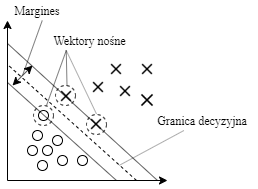
\includegraphics{svm}
\caption{Margines w algorytmie maszyny wektorów nośnych.}
\end{figure}
\section{Przetwarzanie danych}
\tab W tym dziale przyjrzymy się sposobom przetwarzania danych wejściowych tak, aby umożliwić skuteczniejsze rozpoznawanie.
\subsection{Brakujące dane}
\tab Niekiedy badane obiekty nie zawierają np. wartości jakiejś cechy, większość algorytmów nie potrafi sobie poradzić w takiej sytuacji. Narzędzia bibliotek \textit{pandas} oraz \textit{scikit-learn} pozwalają wykrywać takie sytuacje i podejmować konkretne działania.
\begin{itemize}
\item Usuwanie próbek lub cech niezawierających wartości - jednym ze sposobów jest po prostu usunięcie wadliwej próbki lub cechy. Istnieje jednak ryzyko, że usuniemy zbyt wiele próbek lub cech.
\item Uzupełnianie brakujących danych - kolejnym rozwiązaniem jest oszacowanie danych na podstawie pozostałych danych. Jedną z najpopularniejszych metod jest imputacja z użyciem średniej. W tej metodzie wyliczana jest średnia na podstawie całej kolumny cech. Zamiast średniej możemy też użyć mediany lub najczęściej występującej cechy.
\end{itemize}
\subsection{Cechy kategoryzujące}
\tab Często cechy obiektów wejściowych nie są wartościami liczbowymi, w takim przypadku należy rozróżnić dwa rodzaje cech: nominalne i porządkowe. Cechy porządkowe to takie, gdzie możemy ustalić jakąś kolejność, np. rozmiar ubrania XL > L > M > S. Cechy nominalne to na przykład kolor tego ubrania.\\
\tab W przypadku cech porządkowych wystarczy przypisać wartości liczbowe kolejnym cechom, korzystając z poprzedniego przykładu:
XL - 4
L - 3
M - 2
S - 1\\
\tab Z kolei cechom nominalnych nie można po prostu przypisać wartości liczbowej, jest to często popełniany błąd podczas przetwarzania danych wejściowych. Algorytm będzie zakładał, że kolor np. niebieski jest większy od zielonego. Algorytm może generować poprawne wyniki, chociaż będą one dalekie od optymalnych. Rozwiązaniem jest kodowanie gorącojedynkowe, pod tą nazwą kryje się tworzenie sztucznych cech dla każdej nominalnej wartości. Tabela 4.1 przedstawia kodowanie trzech kolorów dla trzech próbek.
\begin{table}[H]
\centering
\caption{Kodowanie gorącojedynkowe cech nominalnych}
\begin{tabular}{c|c|c|c}

indeks & niebieski & czerwony & zielony \\
\hline
0 & 0 & 1 & 0 \\
\hline
1 & 0 & 0 & 1 \\
\hline
2 & 1 & 0 & 0 \\

\end{tabular}
\end{table}
Z tabeli 4.1 możemy odczytać, że ubranie o indeksie 0 ma kolor czerwony, indeksie\linebreak 1 zielony, a indeksie 2 niebieski.
\subsection{Kodowanie etykiet klas}
\tab Zazwyczaj dane wejściowe posiadają etykiety klas zakodowane w postaci nieliczbowej, np. w przypadku tej pracy są to nazwy epok z których pochodzi dany utwór. Dobrym zwyczajem jest przekształcenie nazw etykiet na wartości liczbowe. To jakie wartości przyjmą nie ma znaczenia dla algorytmu, muszą być po prostu unikatowe dla danej etykiety. Zazwyczaj etykiety są numerowane od zera. 
\subsection{Dane uczące i dane testowe}
\tab Nasz zbiór danych należy podzielić na dane uczące, czyli te które będą kształtowały model i testowe, czyli przeciw którym będzie model sprawdzany. Rezygnujemy wtedy\linebreak z części informacji, więc nie możemy umieszczać zbyt wielu próbek w zbiorze testowym. Nie ma dokładnej proporcji podziału danych i zależy ona od wielkości zbioru. Najczęściej są to stosunki 60:40, 70:30, 80:20 lub w przypadku w użytych zbiorów są spotykane wartości takie jak 90:10 lub 99:1.
\subsection{Skalowanie cech}
\tab Skalowanie cech polega na sprowadzeniu wszystkich cech do jednej skali co przyspiesza działanie algorytmów uczenia maszynowego. Najpopularniejsze dwie metody skalowania cech to normalizacja i standaryzacja. Aby przeprowadzić normalizację wystarczy przeskalować każdą kolumnę cech wobec wartości krańcowych ze wzoru:\\
\begin{equation}
x^{(i)}_{norm} = \dfrac{x^{(i)}-x_{min}}{x_{max}-x_{min}}
\end{equation}
Standaryzację kolumny można przeprowadzić wykorzystując wzór:\\
\begin{equation}
x^{(1)}_{std} = \dfrac{x^{(i)} - \mu_x}{\sigma_x}
\end{equation}
\subsection{Dobór cech}
\tab Częstym problemem jest tak zwane nadmierne dopasowanie modelu, czyli sytuacja kiedy model zbyt mocno dopasowany jest do danych uczących, co negatywnie wpływa na wyniki predykcji podczas użycia rzeczywistych zbiorów danych. Taki model cechuje duża wariancja. Przyczynami takich wyników jest zbyt duża złożoność modelu, a problem ten można rozwiązać poprzez: większą ilość danych uczących, karę za złożoność, prostszy model lub zmniejszenie wymiarowości danych.
\chapter{Implementacja aplikacji}
\section{Środowisko}
\tab Aplikacja została napisana przy użycia języka programowania Python w wersji 3.6 oraz zewnętrznych bibliotek do tego języka. Poza standardowymi bibliotekami języka Python użyto:
\begin{itemize}
\item \textit{NumPy} - biblioteka umożliwiająca szybkie operacje na macierzach wielowymiarowych,
\item \textit{Pandas} - dostarcza zoptymalizowane i łatwe w obsłudze struktury danych, które są kompatybilne z narzędziami biblioteki \textit{NumPy},
\item \textit{scikit-learn} - biblioteka umożliwiająca klasyfikację obiektów na podstawie uczenia maszynowego, jest kompatybilna z narzędziami dostarczanymi przez \textit{NumPy} oraz \textit{Pandas},
\item \textit{music21} - zestaw narzędzi do analizy różnych formatów muzycznych, między innymi MIDI oraz MusicXML, pozwala również na pisanie własnych utworów w języku Python.
\end{itemize}
\section{Biblioteka music21}
\tab Dzięki prostemu interfejsowi biblioteki \textit{music21} w bardzo łatwy sposób można odczytywać informacje z plików MusicXML.
\begin{lstlisting}
import music21

stream = music21.converter.parse("C:\\sciezka\\do\\pliku.mxl")
\end{lstlisting}
\tab Powyższy kod tworzy obiekt typu \textit{Stream} zawierający wszystkie informacje przechowywane w pliku MusicXML, a także udostępnia metody pozwalające na działanie na tym obiekcie. 
\subsection{Parametryzacja plików}
\tab Następujące parametry zostały pozyskane z plików muzycznych i były używane do stworzenia danych wejściowych dla algorytmów uczenia maszynowego:
\begin{itemize}
\item średnia wysokość dźwięku,
\item średnia wysokość dźwięku ważona czasem trwania dźwięku,
\item odchylenie standardowe wysokości dźwięku,
\item średnia długość dźwięku,
\item odchylenie standardowe długości dźwięku,
\item znormalizowana liczba nut ze względu na wysokość dźwięku,
\item znormalizowana liczba nut ze względu na czas trwania dźwięku.
\end{itemize}
\subsection{Implementacja parametryzacji plików}
\tab Została napisana klasa \textit{StreamAnalyzer}, która przyjmuje dwa argumenty podczas tworzenia obiektu - \textit{stream} oraz \textit{era}. Argument \textit{stream} to obiekt typu \textit{music21.Stream}, czyli Python'owa reprezentacja pliku muzycznego, a \textit{era} oznacza epokę z której ten plik pochodzi (argument wymagany do tworzenia bazy danych). Klasa \textit{StreamAnalyzer} zawiera pola, z wyżej wymienionymi parametrami, które są pozyskiwane bezpośrednio z obiektu \textit{Stream} przy pomocy metody klasy \textit{StreamAnalyzer} - \textit{extract\_parameters()}, która znajduje się poniżej.\\
\tab Lista zawierająca wszystkie nuty w utworze tworzona jest przez prywatną metodę klasy \textit{StreamAnalyzer} \textit{\_flatten\_stream()}, która łączy wszystkie części utworu w jeden\linebreak i zbiera wszystkie nuty w jedną listę, która dalej jest przetwarzana.
\begin{lstlisting}
def extract_parameters(self) -> None:
    """
    Method that calculates parameters from list of notes
    """
    pitch_frequencies = [note.pitch.frequency
                        for note in self.notes_in_stream]
    weighted_pitch_frequencies = \
    	[note.pitch.frequency * note.duration.quarterLength
        for note in self.notes_in_stream]
    notes_durations = \
      [note.duration.quarterLength
        if not isinstance(
        note.duration.quarterLength, fractions.Fraction)
        else note.duration.quarterLength.numerator / \
            note.duration.quarterLength.denominator
        for note in self.notes_in_stream]
    self.avg_pitch_freq = np.average(pitch_frequencies)
    self.weighted_avg_pitch_freq = \
        np.average(weighted_pitch_frequencies)
    self.pitch_std = np.std(pitch_frequencies)
    self.avg_note_duration = np.average(notes_durations)
    self.note_duration_std = np.std(notes_durations)
    self.notes_by_pitch = Counter(pitch_frequencies)
    self.notes_by_duration = Counter(notes_durations)
    self.name = self.stream.filePath.stem
\end{lstlisting}
\tab Metoda nie przyjmuje żadnych argumentów. Na początku tej metody tworzone są listy wysokości dźwięków w utworze, ważonych wysokości dźwięków w utworze, gdzie wagą jest długość dźwięku oraz lista długości dźwięków w utworze. W kolejnym kroku obliczane i przypisywane do pól obiektu są parametry. Obliczenia wykonywane są przy pomocy biblioteki \textit{NumPy} oraz obiektu \textit{Counter} należącego do biblioteki standardowej \textit{collections}. Obiekt \textit{Counter} pozwala w prosty sposób policzyć liczbę występowania danej wartości w liście. Na koniec do obiektu przypisywana jest też nazwa pliku.\\
\tab W ten sposób tworzone są obiekty zawierające już tylko przydatne informacje. 
\section{Tworzenie DataFrame oraz bazy CSV}
\tab Kolejnym etapem jest przetworzenie listy obiektów typu \textit{StreamAnalyzer} zawierających informacje o utworach muzycznych w jedną pełną bazę danych. Służy do tego klasa znajdująca się w pliku \textit{data\_parser.py} o tej samej nazwie \textit{DataParser}. Metody klasy \textit{DataParser} pozwalają na stworzenie jednego dużego słownika zawierającego informacje o utworach, przekształcenie go tak, aby miał tylko twa wymiary, ponieważ parametry "Znormalizowana liczba nut ze względu na wysokość dźwięku" oraz "Znormalizowana liczba nut ze względu na czas trwania dźwięku" wciąż są przechowywane w formie słowników. Przekształcenie pozwala na stworzenie nowych cech na podstawie każdego klucza z owych słowników - zamiast dwóch parametrów tworzy się ich wiele w zależności od tego ile rodzajów nut było w omawianych dwóch parametrach. Robi to metoda klasy \textit{DataParser} o nazwie \textit{flatten\_dictionaries()}, która jednocześnie normalizuje liczbę nut względem wszystkich nut w utworze, tak żeby długość utworu nie miała większego wpływu na wyniki.\\
\tab Metoda \textit{flatten\_dictionaries()} zwraca słownik, z którego tworzony jest obiekt typu \textit{DataFrame} biblioteki \textit{pandas} za pomocą metody \textit{create\_data\_frame()}. Obiekt \textit{DataFrame} może być zapisany (i równie prosto odczytany) bezpośrednio do pliku CSV (ang. \textit{comma seperated values}, czyli formatu pozwalającego do przechowywania uporządkowanych danych w plikach tekstowych. Tak przygotowane dane można przekazać do algorytmów uczenia maszynowego.
\section{Wybieranie parametrów}
\tab Jako, że parametrów dla każdego utworu na tym etapie jest bardzo dużo -  113, należy zatem wybrać te najbardziej znaczące. Z pomocą przychodzi biblioteka \textit{scikit-learn} posiadająca klasę \textit{RandomForestClassifier} w module \textit{ensemble}. Klasa ta dzięki metodzie \textit{fit()} pozwala na estymowanie ważności wag zbioru cech dzięki temu zwiększając celność modelu i kontrolę nadmiernego dopasowania. Na rysunku 5.1 przedstawiono fragment listingu konsoli przedstawiającego 25 pierwszych cech i ich wagi estymowane przez klasę \textit{RandomForestClassifier}.\\
\begin{figure}[!htb]
\centering
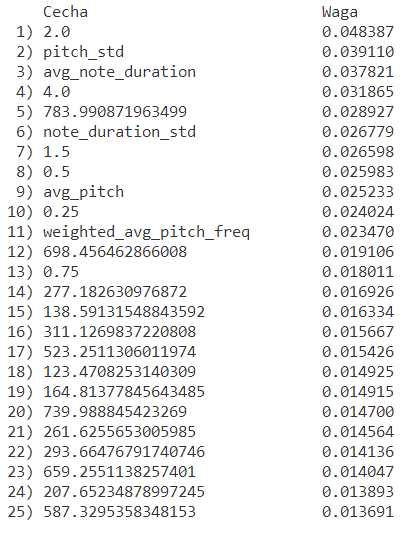
\includegraphics{wagi}
\caption{Fragment konsoli pokazujący znaczenie wagi cech.}
\end{figure}
\tab We wszystkich powtórzeniach na pierwszym miejscu zawsze znajdywały się cechy: 
\begin{itemize}
\item 2.0 - ilość nut o długości dwóch pełnych nut,
\item pitch\_std - odchylenie standardowe wysokości dźwięku,
\item avg\_note\_duration - średnia długość dźwięku,
\item 4.0 - ilość nut o długości czterech pełnych nut.
\end{itemize}
\tab Na podstawie pierwszych czterech oraz trzynastu cech zostały przetworzone bazy danych i nowe pliki CSV posiadający tylko wybrane cechy.\newpage

\section{Trenowanie modelu}
\tab Posiadając przygotowane dane w prosty sposób można było przygotować model. Biblioteka \textit{scikit-learn} w prosty sposób pozwala podzielić zestaw danych na testowy\linebreak i treningowy przy pomocy funkcji \textit{train\_test\_split()}.
\begin{lstlisting}
params_train, params_test, labels_train, labels_test = \
    train_test_split(params, labels, test_size=test_size,
                     random_state=random_state)
\end{lstlisting}
\tab Argument test\_size odpowiada za stosunek podziału, domyślnie 60:40, gdzie 60\% próbek to próbki testowe. Stosunek ten można zmieniać podczas trenowania modelu używając odpowiedniego argumentu wiersza poleceń, o którym będzie w dalszej części pracy. W kolejnym kroku należy przeprowadzić standaryzację danych testowych i uczących zgodnie ze wzorem 4.2 za co odpowiada klasa \textit{StandardScaler} biblioteki \textit{scikit-learn}.
\begin{lstlisting}
sc = StandardScaler()
sc.fit(params)
params_train_std = sc.transform(params_train)
params_test_std = sc.transform(params_test)
\end{lstlisting}
\tab Zmienne \textit{params\_train\_std} oraz \textit{params\_test\_std} są posiadają ustandaryzowane wartości wykorzystane do uczenia modelu.

\begin{lstlisting}
svc = SVC(kernel=kernel, random_state=random_state, gamma=gamma,
  	   C=C)
svc.fit(X=params_train_std, y=labels_train)
    
predictions = svc.predict(params_test_std)
\end{lstlisting}
\tab Powyższy listing przedstawia inicjalizację obiektu SVC biblioteki \textit{scikit-learn} używającą algorytmu maszyny wektorów nośnych. Funkcja \textit{fit()} jako argumenty przyjmuje ustandaryzowane wartości stworzone w poprzednim kroku oraz odpowiadające im etykiety danych oraz trenuje model. Zmienna \textit{predictions} to lista przewidzianych przez model etykiet na podstawie danych \textit{params\_test\_std} użytych jako argument w metodzie \textit{predict}. Dzięki porównaniu jej ze zmienną \textit{labels\_test} możemy sprawdzić skuteczność modelu dla danych testowych. Na koniec drukujemy do konsoli wyniki trenowania, ile było próbek testowych, ile próbek sklasyfikowano niepoprawnie oraz jakie są dokładności modelu dla danych testowych i uczących.
\section{Interfejs wiersza poleceń}
\tab Aplikacja opiera się o interfejs wiersza poleceń (ang. \textit{command line interface}) i udostępnia następujące komendy:
\begin{itemize}
\item --csv-path [PATH] - jedyny wymagany argument, wskazuje ścieżkę do pliku CSV zawierającego przekształconą bazę danych,
\item --mxml-files [PATH] - ścieżka do folderu z plikami MusicXML, tworzy nową bazę danych z plików MusicXML w miejscu wskazanym przez argument --csv-path,
\item --train - nie przyjmuje żadnych argumentów, jeśli jest podany na nowo tworzony jest model,
\item --test-size [NUMBER] - ułamek grupy testowej z bazy danych, domyślnie 0.4,
\item --kernel [STRING] - wybór jądra modelu, domyślnie "rbf",
\item --gamma [NUMBER] - obszar graniczny strefy Gauss'a, tym większa gamma tym mniej sztywne są granice decyzyjne modelu, domyślnie 0.1, 
\item -C [NUMBER] - odwrotność parametru regularyzacji, zapobiega zbyt dużej wartości wag cech, domyślnie 1.0, 
\item --random-state [STRING or INTEGER] - generator liczb pseudolosowych, jeśli podana jest liczba stała, użyta jest jako ziarno generatora liczb losowych, domyślnie użyty jest generator biblioteki \textit{NumPy},
\item --save-model [PATH] - ścieżka do zapisu modelu, model powinien być zapisany\linebreak z rozszerzeniem \textit{.joblib},
\item --classify [PATH] - ścieżka do zapisanego modelu, jeśli został podany argument --train użyty zostanie aktualny model z pamięci,
\item -h, --help - pomoc, wyświetla informacje o dostępnych argumentach.
\end{itemize}
\subsection{Przykłady użycia}
\begin{lstlisting}
py mxml_recognizer.py \
	--csv-path .\bazy_danych\nowa_baza.csv \
	--mxml-files .\pliki_musicxml 
\end{lstlisting}
Powyższa komenda tworzy nową bazę danych w pliku \textit{nowa\_baza.csv} na podstawie plików znajdujących się w folderze \textit{pliki\_musicxml}.
\begin{lstlisting}
py mxml_recognizer.py \
	--csv-path .\bazy_danych\nowa_baza.csv \
	--train \
	--save-model .\modele\nowy_model.joblib
\end{lstlisting}
Trenuje model na podstawie istniejącej bazy danych 
\textit{nowa\_baza.csv} oraz zapisuje go do pliku \textit{nowy\_model.joblib}.

\begin{lstlisting}
py mxml_recognizer.py \
	--csv-path .\bazy_danych\testowa_baza.csv \
	--classify .\modele\nowy_model.joblib
\end{lstlisting}
Klasyfikuje przetworzone na format CSV pliki z pliku \textit{testowa\_baza.csv}. 
\chapter{Podsumowanie}
\tab Celem pracy inżynierskiej było wykonanie aplikacji do automatycznej klasyfikacji utworów muzycznych ze względu na przynależność do danej epok. Cel został osiągnięty, a wyniki działania aplikacji przedstawiono poniżej.
\section{Wyniki}
\tab Na podstawie bazy danych zawierającej najmniejszą ilość parametrów zostały stworzone, z użyciem biblioteki  \textit{matplotlib}, wykresy słupkowe ze średnią wartością danego parametru dla poszczególnych epok. 
\begin{figure}[H]
\centering
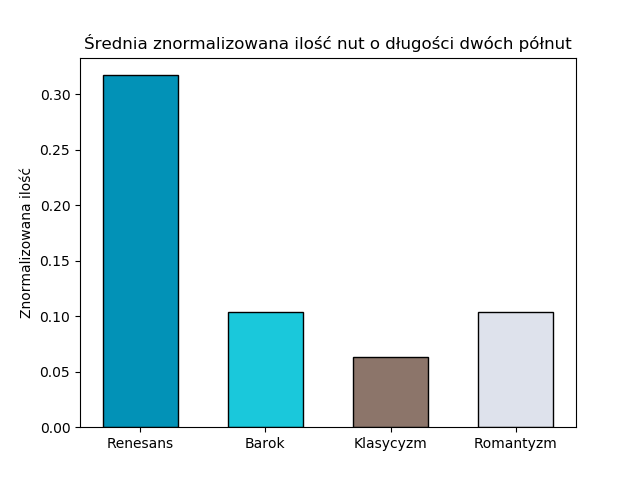
\includegraphics[scale=0.75]{plots/2fullnotes.png}
\caption{Średnia znormalizowana ilość nut o długości dwóch półnut.}
\end{figure}
\begin{figure}[H]
\centering
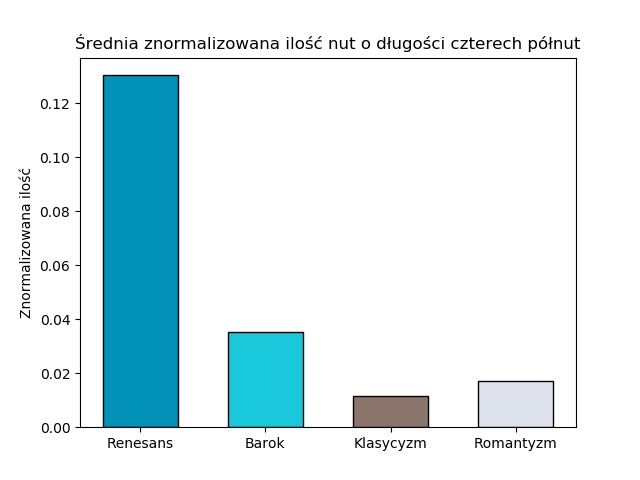
\includegraphics[scale=0.75]{plots/4fullnotes.png}
\caption{Średnia znormalizowana ilość nut o długości czterch półnut.}
\end{figure}
\begin{figure}[H]
\centering
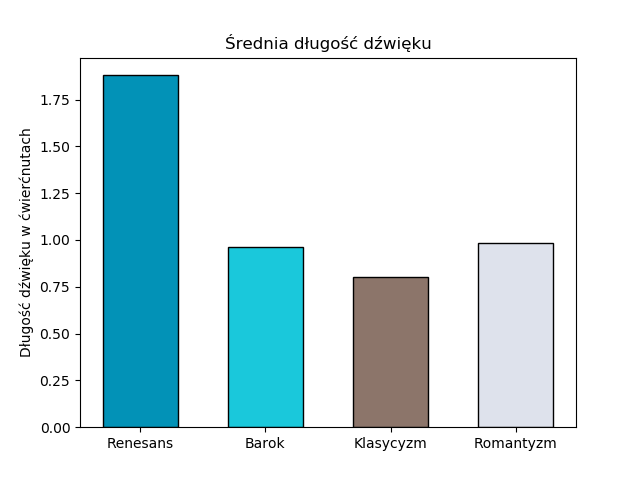
\includegraphics[scale=0.75]{plots/avg_note_dur.png}
\caption{Średnia długość dźwięku.}
\end{figure}
\begin{figure}[H]
\centering
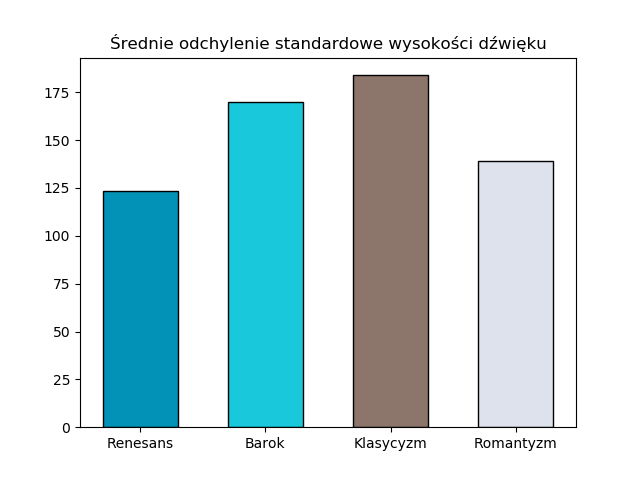
\includegraphics[scale=0.75]{plots/avg_pitch_std.png}
\caption{Średnia odchylenie standardowe wysokości dźwięku.}
\end{figure}

\tab Powyższe wykresy przedstawiają cztery wybrane parametry do ostatecznego modelu. Na podstawie tych czterech parametrów widać, że renesans jest najbardziej dystynktywną epoką, w której nuty mają większe wartości, a dźwięki w mniejszym stopniu zmieniają swoją wysokość. Pozostałe epoki były znacznie bardziej zbliżone do siebie.\\
\tab Poniżej przedstawiono wyniki z konsoli aplikacji dla trenowania modelu przy użyciu bazy danych zawierającej tylko 4 cechy.
\begin{figure}[H]
\centering
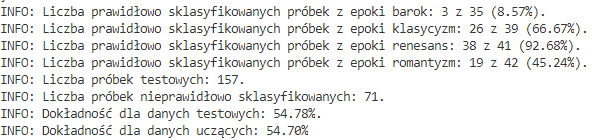
\includegraphics[scale=0.9]{wyniki_smaller_0.png}
\caption{Wyniki trenowania modelu, cztery cechy, powtórzenie pierwsze.}
\end{figure}
\begin{figure}[H]
\centering
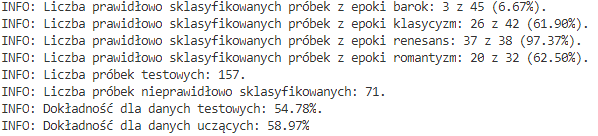
\includegraphics[scale=0.9]{wyniki_smaller_1.png}
\caption{Wyniki trenowania modelu, cztery cechy, powtórzenie drugie.}
\end{figure}
\begin{figure}[H]
\centering
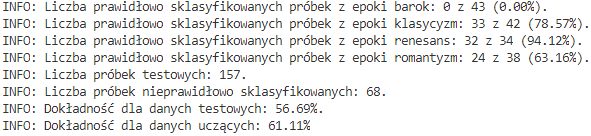
\includegraphics[scale=0.9]{wyniki_smaller_2.png}
\caption{Wyniki trenowania modelu, cztery cechy, powtórzenie trzecie.}
\end{figure}
\tab Najgorzej rozpoznawalną epoką w tym przypadku jest barok, który oscylował\linebreak w okolicy 3\%. Za to renesans był bliski 100\% co również widać z wykresów na rysunkach 6.1, 6.2, 6.3 oraz 6.4, gdzie to renesans jest najbardziej odstający od reszty epok.
\begin{figure}[H]
\centering
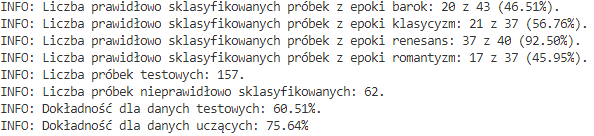
\includegraphics[scale=0.9]{wyniki_small_0.png}
\caption{Wyniki trenowania modelu, trzynaście cech, powtórzenie pierwsze.}
\end{figure}
\begin{figure}[H]
\centering
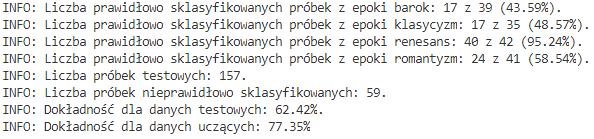
\includegraphics[scale=0.9]{wyniki_small_1.png}
\caption{Wyniki trenowania modelu, trzynaście cech, powtórzenie drugie.}
\end{figure}
\begin{figure}[H]
\centering
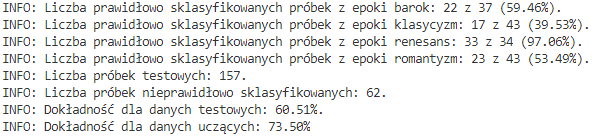
\includegraphics[scale=0.9]{wyniki_small_2.png}
\caption{Wyniki trenowania modelu, trzynaście cech, powtórzenie trzecie.}
\end{figure}
\tab Następnie użyto trzynastu pierwszych cech wskazanych przez listing z rysunku 5.1, wyniki znacznie się zmieniły. Rozpoznawalność baroku wzrosła o ponad 40 punktów procentowych, kosztem rozpoznawalności klasycyzmu oraz romantyzmu. Renesans pozostał bez zmian. Dokładność modelu dla danych uczących znacznie jednak odbiegała od dokładności dla danych testowych. 
\begin{figure}[H]
\centering
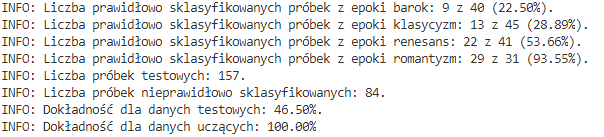
\includegraphics[scale=0.9]{wyniki_all_0.png}
\caption{Wyniki trenowania modelu, sto trzynaście cech, powtórzenie pierwsze.}
\end{figure}
\begin{figure}[H]
\centering
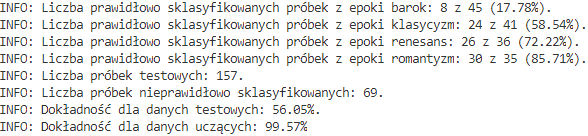
\includegraphics[scale=0.9]{wyniki_all_1.png}
\caption{Wyniki trenowania modelu, sto trzynaście cech, powtórzenie drugie.}
\end{figure}
\begin{figure}[H]
\centering
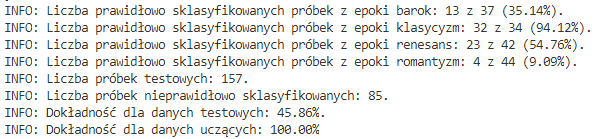
\includegraphics[scale=0.9]{wyniki_all_2.png}
\caption{Wyniki trenowania modelu, sto trzynaście cech, powtórzenie trzecie.}
\end{figure}
\tab Dla porównania użyto też wszystkich stu trzynastu cech. Dokładność danych uczących wynosiła praktycznie 100\%, a testowych około 50\% widać ewidentne przetrenowanie modelu - model zbyt mocno dopasował się do danych uczących co sprawia, że nie radzi sobie z danymi testowymi. Rozpoznawalność dla poszczególnych epok jest losowa i bardzo zależy od wyboru danych do nauki modelu.
\section{Wnioski}
\tab Wybór odpowiednich parametrów jest kluczowym etapem uczenia maszynowego, jak widać po wynikach użycie wszystkich dostępnych cech wcale nie daje najlepszych rezultatów, wręcz przeciwnie, tylko pogarsza wyniki, a model jest dopasowany idealnie tylko do zestawu uczącego. Sytuację tą przedstawia rysunek 6.14. Jak widać na przykładzie z rysunku 6.14 zielona linia idealnie oddziela dwie cechy i w porównaniu do czarnej lepiej radzi sobie z klasyfikacją, jednak dzieje się tak tylko dla danych uczących i dla rzeczywistych danych zielona linia będzie powodowała znacznie większy błąd klasyfikacji niż czarna linia.
\begin{figure}[H]
\centering
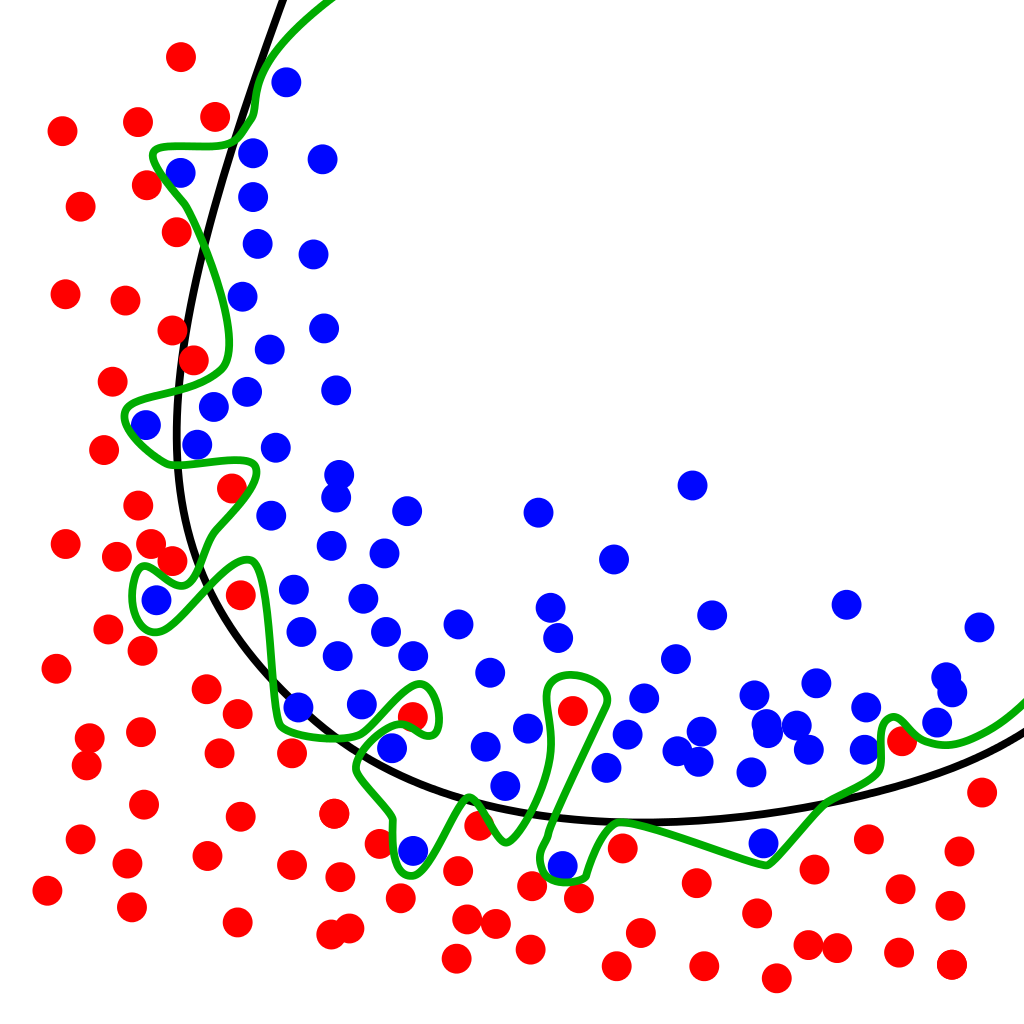
\includegraphics[scale=0.3]{overfitting.png}
\caption{Zielona linia pokazuje zachowanie modelu przetrenowanego, czarna model do którego dążymy.}
\end{figure}
\tab W przypadku użycia tylko 4 cech wskazanych przez klasę \textit{RandomForestClassifier} znacznie zmalała rozpoznawalność epoki barokowej. Z kolei użycie 13 pierwszych parametrów było najbardziej optymalnym, jednak wciąż niezadowalającym rozwiązaniem.\\
\tab Niepowiedziane też jest, że można rozpoznawać klasyczne utwory muzyczne na tylko na podstawie wybranych w tej pracy cech. Sprawę komplikuje też fakt, że artyści nie zawsze trzymali się jednej formy, a ich utwory niekiedy bardzo zmieniały się w ciągu okresu twórczości, czasami wychodząc stylem poza swoją epokę, przykładem może być twórczość Beethoven'a, którego ciężko sklasyfikować jednoznacznie do klasycyzmu czy romantyzmu.
\tab Praca nad aplikacją zdecydowanie była źródłem cennej wiedzy programistycznej na temat uczenia maszynowego oraz jego implementacji.
\section{Możliwości rozwoju}
\tab Do poprawienia skuteczności klasyfikacji na pewno trzeba przeanalizować inne parametry i znaleźć takie, które znacznie lepiej opisują daną epokę i pozwalają odróżniać ją od pozostałych. Należałoby również poszerzyć bazę danych utworów, być może wykorzystać inne algorytmy uczenia maszynowego. Zagadnienie klasyfikacji klasycznych utworów na pewno nie jest proste. Jeśli chodzi o sam interfejs aplikacji warto dodać możliwość wprowadzenia pojedynczego utworu i jego automatycznej klasyfikacji zamiast całych baz danych.
\end{document}